\begin{frame}
	\textbf{Rising wage inequality}\medskip

	\begin{itemize}\setlength\itemsep{1em}
		\item changes in distribution of skills
		\item changes in relative prices of skills, prices identical across sectors
		\item comparative advantage, different skills priced different across sectors $\Longrightarrow$ Roy models
	\end{itemize}
\end{frame}

\begin{frame}
	\begin{itemize}\setlength\itemsep{1em}
		\item Does the pursuit of comparative advantage increase or decrease earnings inequality within sectors and in the overall economy?
		\item Do the people with the highest $i$ skill actually work in sector $i$?
		\item As people enter a sector in response to an increase in the demand for its services, does the average skill level employed there rise or fall?
	\end{itemize}
\end{frame}
%-------------------------------------------------------------------------------
%-------------------------------------------------------------------------------
\begin{frame}
	\textbf{\citeA{Roy.1951} Model}\medskip
	\begin{itemize}\setlength\itemsep{1em}
		\item Individuals are income maximizing, act under perfect information, and possess skills $S_1$ and $S_2$.
		\item The economy offers two employment opportunities associated with skill prices $\pi_1$ and $\pi_2$ and skill $i$ is only useful in sector $i$.
	\end{itemize}\medskip
	An individual chooses sector one if earnings are greater there:
	\begin{align*}
	w_1 > w_2 \quad\Longleftrightarrow\quad \pi_1 S_1 > \pi_2 S_2
	\end{align*}
\end{frame}

%-------------------------------------------------------------------------------
%-------------------------------------------------------------------------------
\begin{frame}
\begin{figure}[htp]\centering
\scalebox{0.40}{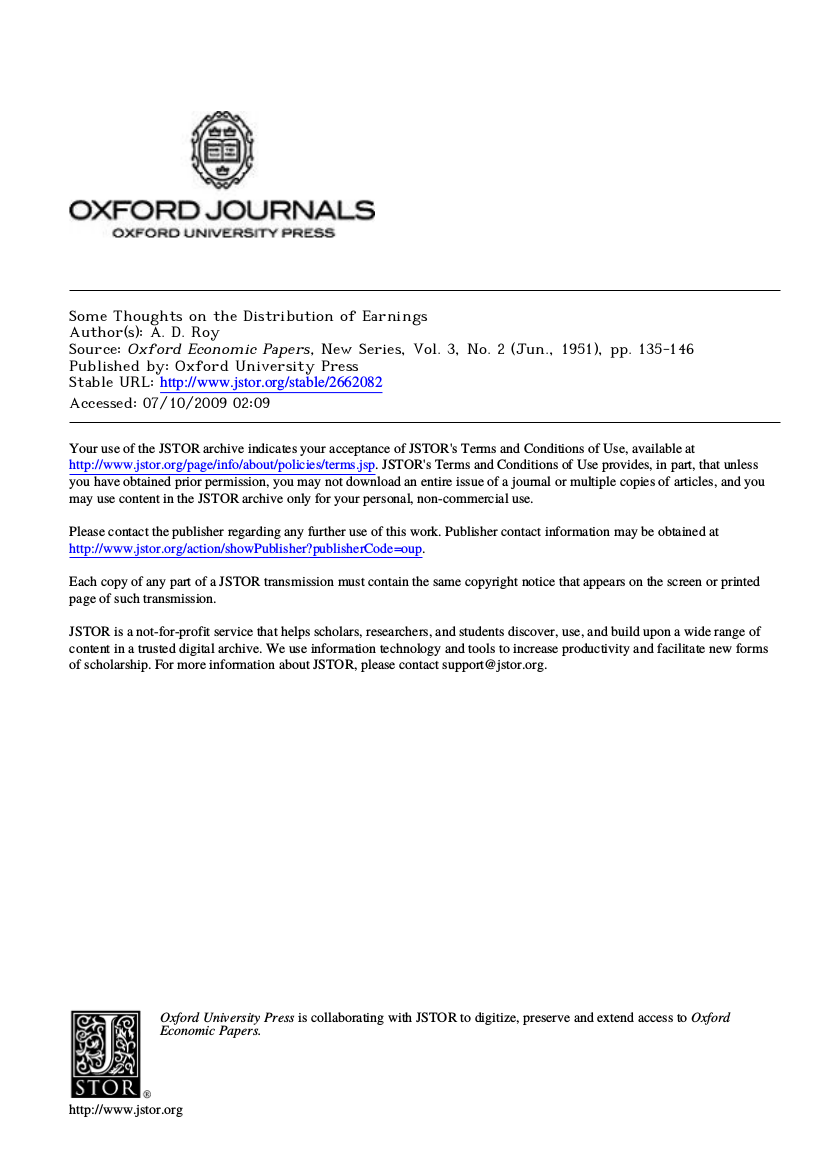
\includegraphics{fig-cover-roy-1951}}
\end{figure}
\end{frame}
